\chapter{Řízení DBS projektu} \label{DBSmanagement}

Tato kapitola popisuje řízení DBS projektu z hlediska lidských zdrojů, komunikace a použitých technologií.

// TODO smth

\section{Řízení lidských zdrojů}

Řízení lidských zdrojů je jednou z neobtížnějších součástí projektového řízení, především proto, že se prolíná s dalšími odvětvími jako například \emph{psychologií} či \emph{sociologií}. Jelikož lidé jsou hnací silou projektu, mohou různé metody či samotná kvalita (ba dokonce absence!) řízení lidských zdrojů odrážet výsledný úspěch či neúspěch projektu. I v DBS projektu tedy vyvstala potřeba tuto pozici zaujmout a chopil jsem se jí já, jak již bylo popsáno v kapitole \ref{intro:me}.

\subsection{Role psychologie v řízení lidí}
Ještě než se ponoříme do samotných procesů popisujících řízení lidkých zdrojů, věnujme se chvíli právě oněm dalším odvětvím, které se s řízením lidí prolínají. Jak již bylo řečeno, jedná se především o \emph{psychologii}.

Lidé nejsou stroje, kterým poskytneme určitý vstup a podle jeho množství můžeme očekávat výstup. Je potřeba se zamýšlet nad dalšími okolnostmi, proč pro nás daný člověk pracuje, zda je spokojený, kdy odvádí nejlepší práci atp. Za veškerou lidskou činností stojí \emph{nějaká} motivace, cílem projektového manažera je poté najít, co motivuje právě jemu svěřené pracovníky.

\paragraph{\nameref{picture:maslow}}
\begin{figure}[h]
	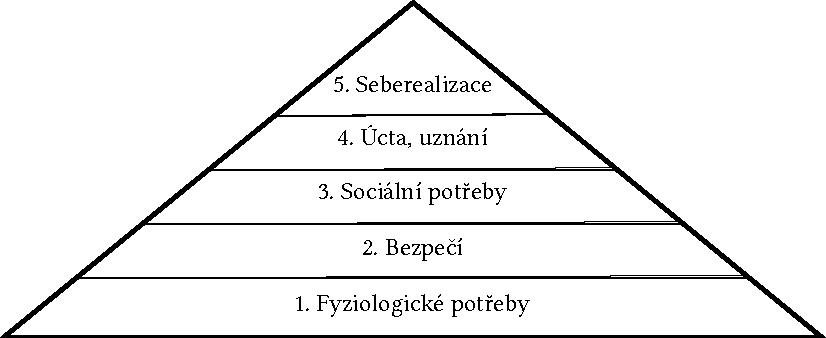
\includegraphics{../pdf/maslow.pdf}
	\caption{Maslowova pyramida potřeb} \label{picture:maslow}
\end{figure}

Ve standardních projektech, kde jsou vývojáři odměňováni finančne, se dá plat považovat za splnění základních fyziologických potřeb, protože je za něj možné nakoupit právě jídlo či pití. V DBS projektu jsou namísto finančně studenti hodnoceni známkou z předmětu, který je pro jejich studijní obor povinný. Jelikož však \emph{vystudování vysoké školy} obecně je spíše potřebou \emph{úcty, uznání} či \emph{seberealizace}, jedná se o vyšší patra pyramidy. Maslow tvrdí, že není možné uspokojovat vyšší patra pyramidy, pokud nejsou zajištěny ty nižší. Z toho důvodu může být obtížné motivovat k práci ty studenty, kteří nejprve potřebují vyřešit své zabezpečení (1. a 2. úroveň pyramidy), takoví studenti budou logicky dávat přednost před prací na projektu opravdové práci, za kterou dostanou peníze. Jakmile však má student zajíštěné tyto \uv{nižší potřeby}, dostávají se do popředí právě ty, které může DBS projekt nabídnout. Toto otevírá skvělé možnosti pro rozvoj jak samotných studentů, tak výsledného portálu. Jako příklad uvedu Pavla Kováře, který v tuto chvíli pracuje na bakalářské práci na téma \emph{Automatizované testování webového portálu dbs.fit.cvut.cz}. K projektu se dostal stejnou cestou jako já, ale o rok později. Po dokončení předmětu BI-SP2 se rozhodl u projektu zůstat a pokračovat v jeho vývoji. Jelikož již během vývoje v rámci SP týmů sám od sebe přicházel s inovacemi a kvalitními návrhy na zlepšení, jedná se dle mého názoru o jasný příklad naplňování nejvyšší potřeby, a to \emph{seberealizace}.\\
Právě seberealizace je jedna z potřeb, na kterou se snažím při řízení DBS projektu klást důraz. Studenti jsou hodnoceni jednak za práci, která je jim zadána, navíc ale dostávají příležitosti rozvíjet vlastní nápady a přínosy projektu a jsou za tyto přínosy také kladně hodnoceni. Více o hodnocení je popisováno v sekci TODO.

\subsection{Procesy řízení lidských zdrojů}

Jak popisuje Schwalbe \cite{schwalbe} ve své knize \emph{Řízení projektů v IT: kompletní průvodce}, při řízení lidských zdrojů se rozeznávají následující procesy:

\subsubsection{Vytvoření plánu lidských zdrojů}

Tento proces, jak název vypovídá, se u typických projektů řeší 


\paragraph{Použití v DBS projektu}
TODO
